\RequirePackage{docswitch}
% \flag is set by the user, through the makefile:
%    make note
%    make apj
% etc.
\setjournal{\flag}

\documentclass[twocolumn]{\docclass}

%%%% Scott's macros
\newcommand{\sfig}[2]{
\includegraphics[width=#2]{#1}
        }
\newcommand{\Sfig}[2]{
    \begin{figure}[thbp]
    \sfig{../Figures/#1.pdf}{\columnwidth}
    \caption{{\small #2}}
    \label{fig:#1}
    \end{figure}
}
\newcommand{\Swide}[2]{
\begin{figure*}[thbp]
 \sfig{../Figures/#1.pdf}{.8\textwidth}
  \caption{{\small #2}}
   \label{fig:#1}
   \end{figure*}
}
\newcommand{\Sswide}[2]{
\begin{figure*}[thbp]
 \sfig{../Figures/#1.pdf}{.7\textwidth}
  \caption{{\small #2}}
   \label{fig:#1}
   \end{figure*}
}
\newcommand{\Svwide}[2]{
\begin{figure*}[thbp]
 \sfig{../Figures/#1.pdf}{\textwidth}
  \caption{{\small #2}}
   \label{fig:#1}
   \end{figure*}
}

\newcommand{\Spng}[2]{
    \begin{figure}[thbp]
    \sfig{../Figures/#1.png}{0.95\columnwidth}
    \caption{{\small #2}}
    \label{fig:#1}
    \end{figure}
}
\newcommand{\Rf}[1]{\ref{fig:#1}}
\newcommand{\rf}[1]{\ref{fig:#1}}
\newcommand{\ec}[1]{Eq.~(\ref{eq:#1})}
\newcommand{\ecalt}[1]{Eq.~\ref{eq:#1}}
\newcommand{\Ec}[1]{(\ref{eq:#1})}
\newcommand{\eeec}[3]{Eqs.~(\ref{eq:#1}, \ref{eq:#2}, \ref{eq:#3})}
\newcommand{\eql}[1]{\label{eq:#1}}
\newcommand\be{\begin{equation}}
\newcommand\ee{\end{equation}}
\def\bea{\begin{eqnarray}}
\def\eea{\end{eqnarray}}
% \def\bea{\begin{eqnarray}}
% \def\eea{\end{eqnarray}}
\def\svs{\nonumber\\}

% You could also define the document class directly
%\documentclass[]{emulateapj}

% Custom commands from LSST DESC, see texmf/styles/lsstdesc_macros.sty
\usepackage{lsstdesc_macros}

\usepackage{graphicx}
\graphicspath{{./}{./figures/}}
\bibliographystyle{apj}

% Add your own macros here:



% ======================================================================

\begin{document}

\title{Covariance Testing}

\maketitlepre

\begin{abstract}

There are a number of codes that compute covariance matrices analytically; the plan is to use these to build TJPCov. In this project, we start along the path of comparing these different codes, building up a suite of tools that can be used to compare covariance matrices. We expect these tools to be useful not only for converging on a single accurate code for computing covariance matrices but also more generally for understanding which parts of the covariance matrix carry the most information (and therefore need the most attention to get right) and which are not relevant (so for example matrices that are not positive definite may still be usable if the negative eigenmodes are not relevant).
\end{abstract}

% Keywords are ignored in the LSST DESC Note style:
\dockeys{}

\maketitlepost

% ----------------------------------------------------------------------
% 

\section{Introduction}
\label{sec:intro}


% ----------------------------------------------------------------------

\section{Methods}
\label{sec:methods}

To illustrate our methodology, we use cosmic shear statistics $\xi_\pm(\theta)$, focusing for the most part on the Year 1 results of the Dark Energy Survey~\citep{Abbott:2017wau} (DESY1), and also on predictions for DES Year 3 (DESY3). The data is divided into four tomographic redshift bins spanning the interval $0.20 - 1.30$, which gives us 10 bin combinations, each one containing 20 angular bins between 2.5 and 250 arcmin. We thus have 200 data points for each $\xi_+(\theta)$ and $\xi_-(\theta)$, giving us 400 in total. 

We apply the angular cuts described in ~\citep{Abbott:2018cms}, which removes the scales most sensitive to baryonic effects; this leaves us with 167 points for $\xi_+(\theta)$ and 60 for $\xi_-(\theta)$ (for which baryonic interactions are more relevant), resulting in 227 data, which correspond to a $227 \times 227$ covariance matrix.

The two codes employed here for computing the covariance matrices are {\tt Cosmolike}~\citep{Krause:2016jvl} and a simpler version of the code used to analyze the KiDS-450 survey~\citep{Kohlinger:2017sxk}, hereafter referred to as CL and BJ, respectively. To perform cosmological parameter inference we use the {\tt CosmoSIS}~\citep{ZUNTZ201545} pipeline, while employing the {\tt MultiNest}~\citep{nested:feroz09} sampler to explore the parameter space, with 500 {\tt livepoints}, {\tt efficiency} set to 0.3, {\tt tolerance} to 0.1 and {\tt constant efficiency} set to False.

\begin{table}
\centering
\begin{tabular} { l c} 
\hline
\hline
Parameter							& Prior	\\ \hline
Cosmological & \\ [1ex]
$\Omega_m$						& $\mathcal{U}(0.1, 0.9)$		\\
$A_s \times 10^9$					& $\mathcal{U}(0.5, 5)$		\\
$H_0 \mathrm{(km s^{-1} Mpc^{-1})}$	& $\mathcal{U}(55, 91)$		\\
$\Omega_b$						& $\mathcal{U}(0.03, 0.07)$	\\
$\Omega_\nu h^2$					& $\mathcal{U}(0.0005, 0.01)$	\\
$n_s$							& $\mathcal{U}(0.87, 1.07)$	\\ [1ex]
\hline
Astrophysical & \\ [1ex]
$A$								& $\mathcal{U}(-5, 5)$ \\
$\eta$							& $\mathcal{U}(-5, 5)$ \\ [1ex]
\hline
Systematic & \\ [1ex]
$m^i$							& $\mathcal{G}(0.012, 0.023)$	 \\
$\Delta z^1$						& $\mathcal{G}(-0.001, 0.016)$	 \\
$\Delta z^2$						& $\mathcal{G}(-0.019, 0.013)$	 \\
$\Delta z^3$						& $\mathcal{G}(0.009, 0.011)$	 \\
$\Delta z^4$						& $\mathcal{G}(-0.018, 0.022)$	 \\ [1ex]
\hline
\hline
\end{tabular}
\caption{List of the priors used in the analysis for parameter constraints. For the cosmological parameters, we fixed $w = -1.0$, $\Omega_k =  0.0$ and $\tau =  0.08$. The astrophysical parameters are associated with the intrinsic alignment, they follow the relation $A(z) = A[(1+z)/1.62]^{\eta}$, we have also $z_0 = 0.62$. Lastly, for systematics we have $m^i$ corresponding to the shear calibration, and  $\Delta z^i$ for the source photo-$z$ shift, with $i = 1, 4$ in both cases. The lens photo-$z$ shift parameters $\Delta z^i$, $i = 1, 5$ were fixed to zero.}
\label{tab:constraints}
\end{table}

\subsection{One-to-one Comparison}

This is a simple matter of comparing elements of a covariance matrix, usually starting with diagonal elements. \figref{xipmscatter} shows an example.

\begin{figure}
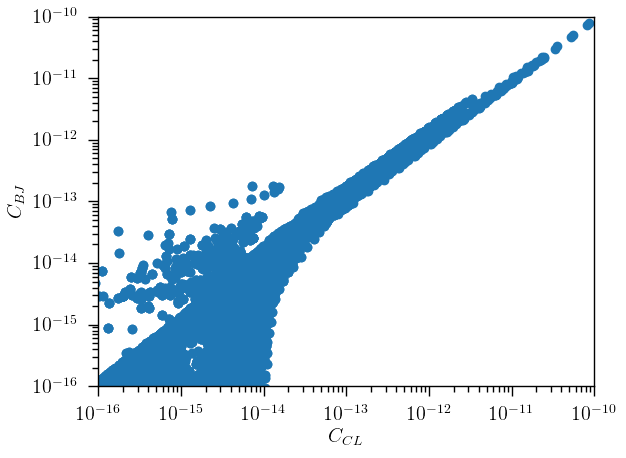
\includegraphics[width=0.9\columnwidth]{xipmscatter.png}
\caption{A simple scatter plot of elements of covariance matrices produced by two separate halo model codes. \label{fig:xipmscatter}}
\end{figure}


\subsection{Eigenvalues and eigenvectors}

An intuitive approach to identifying the most contributing elements of a covariance matrix is to look at its eigenvalues, since we can associate them to the variance. The lowest eigenvalues would correspond to the least variance and therefore hold the most information, whereas the highest eigenvalues would implicate larger error and thus contribute significantly less. With this in mind, the most important elements of the matrix would be those with the lowest eigenvalues. To verify this assumption, we need to look at the parameter constraints: removing the elements with the highest eigenvalues should not alter our results; the opposite, however, should give us a broader constraints. Our procedure consists of first diagonalising the covariance matrix in order to calculate its eigenvalues and then replacing the 50 highest with numbers of about nine orders of magnitude higher, thus removing their effective contribution; we then obtain a new covariance matrix with the modified eigenvalues. We also apply this method to the 50 lowest eigenvalues of the original covariance matrix, and replace them with higher values. Finally, we perform a cosmological analysis with the new covariances matrices, to constrain the parameters of our model. In Figure~\rf{eigenvalues} we compare the results of both approaches to those obtained with the original covariance matrix, for brevity we show only $\Omega_m$ and $\sigma_8$. We can see in the Posterior Density Functions (pdfs) that the mean values of both parameters are well within the $2\sigma$ interval, and this is also true for all the other parameters; the size of the constraints is also within less than 5\% of each other for almost all of the parameters. Since the constraints are similar for both approaches, it becomes clear that ranking eigenvalues is not the most efficient way of evaluating where the most contributing elements of the covariance matrix lie.


\begin{figure}
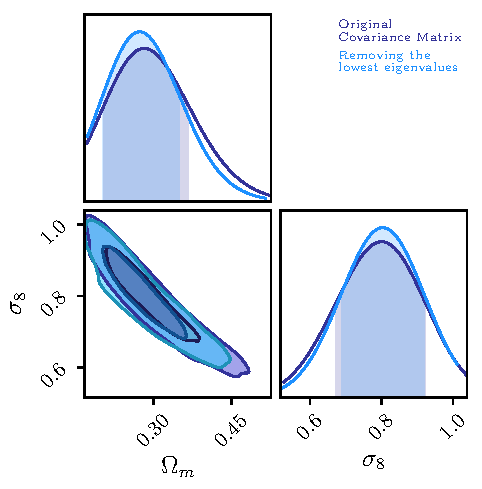
\includegraphics[width=0.9\columnwidth]{Eigenvalues.pdf}
\caption{Constraints on cosmological parameters $\Omega_m$ and $\sigma_8$ for the original DESY1 covariance matrix (in purple) and for two new covariance matrices obtained by setting the fifty highest eigenvalues of the original matrix to nine orders of magnitude higher (in blue), and by replacing the fifty lowest eigenvalues to nine order of magnitude lower (in magenta). \label{fig:eigenvalues}}
\end{figure}


Next, we wish to compare matrices using their eigenvalues. We plot the results obtained for constraints on $\Omega_m$ and $\sigma_8$ for BJ and CL in Figure~\rf{y3-comparison}, where we can see that, while their best fit values agree within a $2 \sigma$ interval, the constraints are up to $25 \%$ broader for the latter. This is also true for the other parameters, where, on average, constraints obtained with CL are about $18 \%$ wider. To see if we can identify these differences in the eigenvalues of the covariance matrices, we plot Figure~\rf{coveigen}. At a first glance, both curves show reasonable agreement, with values differing only by an average of $\approx 15 \%$, but we should keep in mind that the order of magnitude of the values vary greatly, which makes it difficult to compare them efficiently with this methodology. Furthermore, from our previous analysis it is not clear which elements are most important.


\begin{figure}
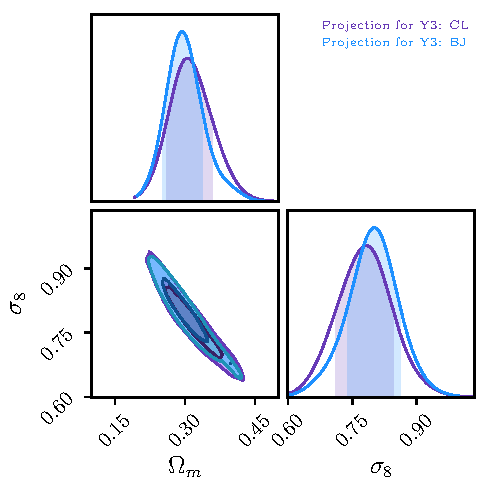
\includegraphics[width=0.9\columnwidth]{Y3-comparison.pdf}
\caption{Constraints on cosmological parameters $\Omega_m$ and $\sigma_8$ for two covariance matrices produced for cosmic shear for DESY3. The purple curve is for CL while the blue is for BJ. The constraints are about $18 \%$ broader for the former, indicating that the two matrices have quantifiable differences between them. \label{fig:y3-comparison}}
\end{figure}

\begin{figure}
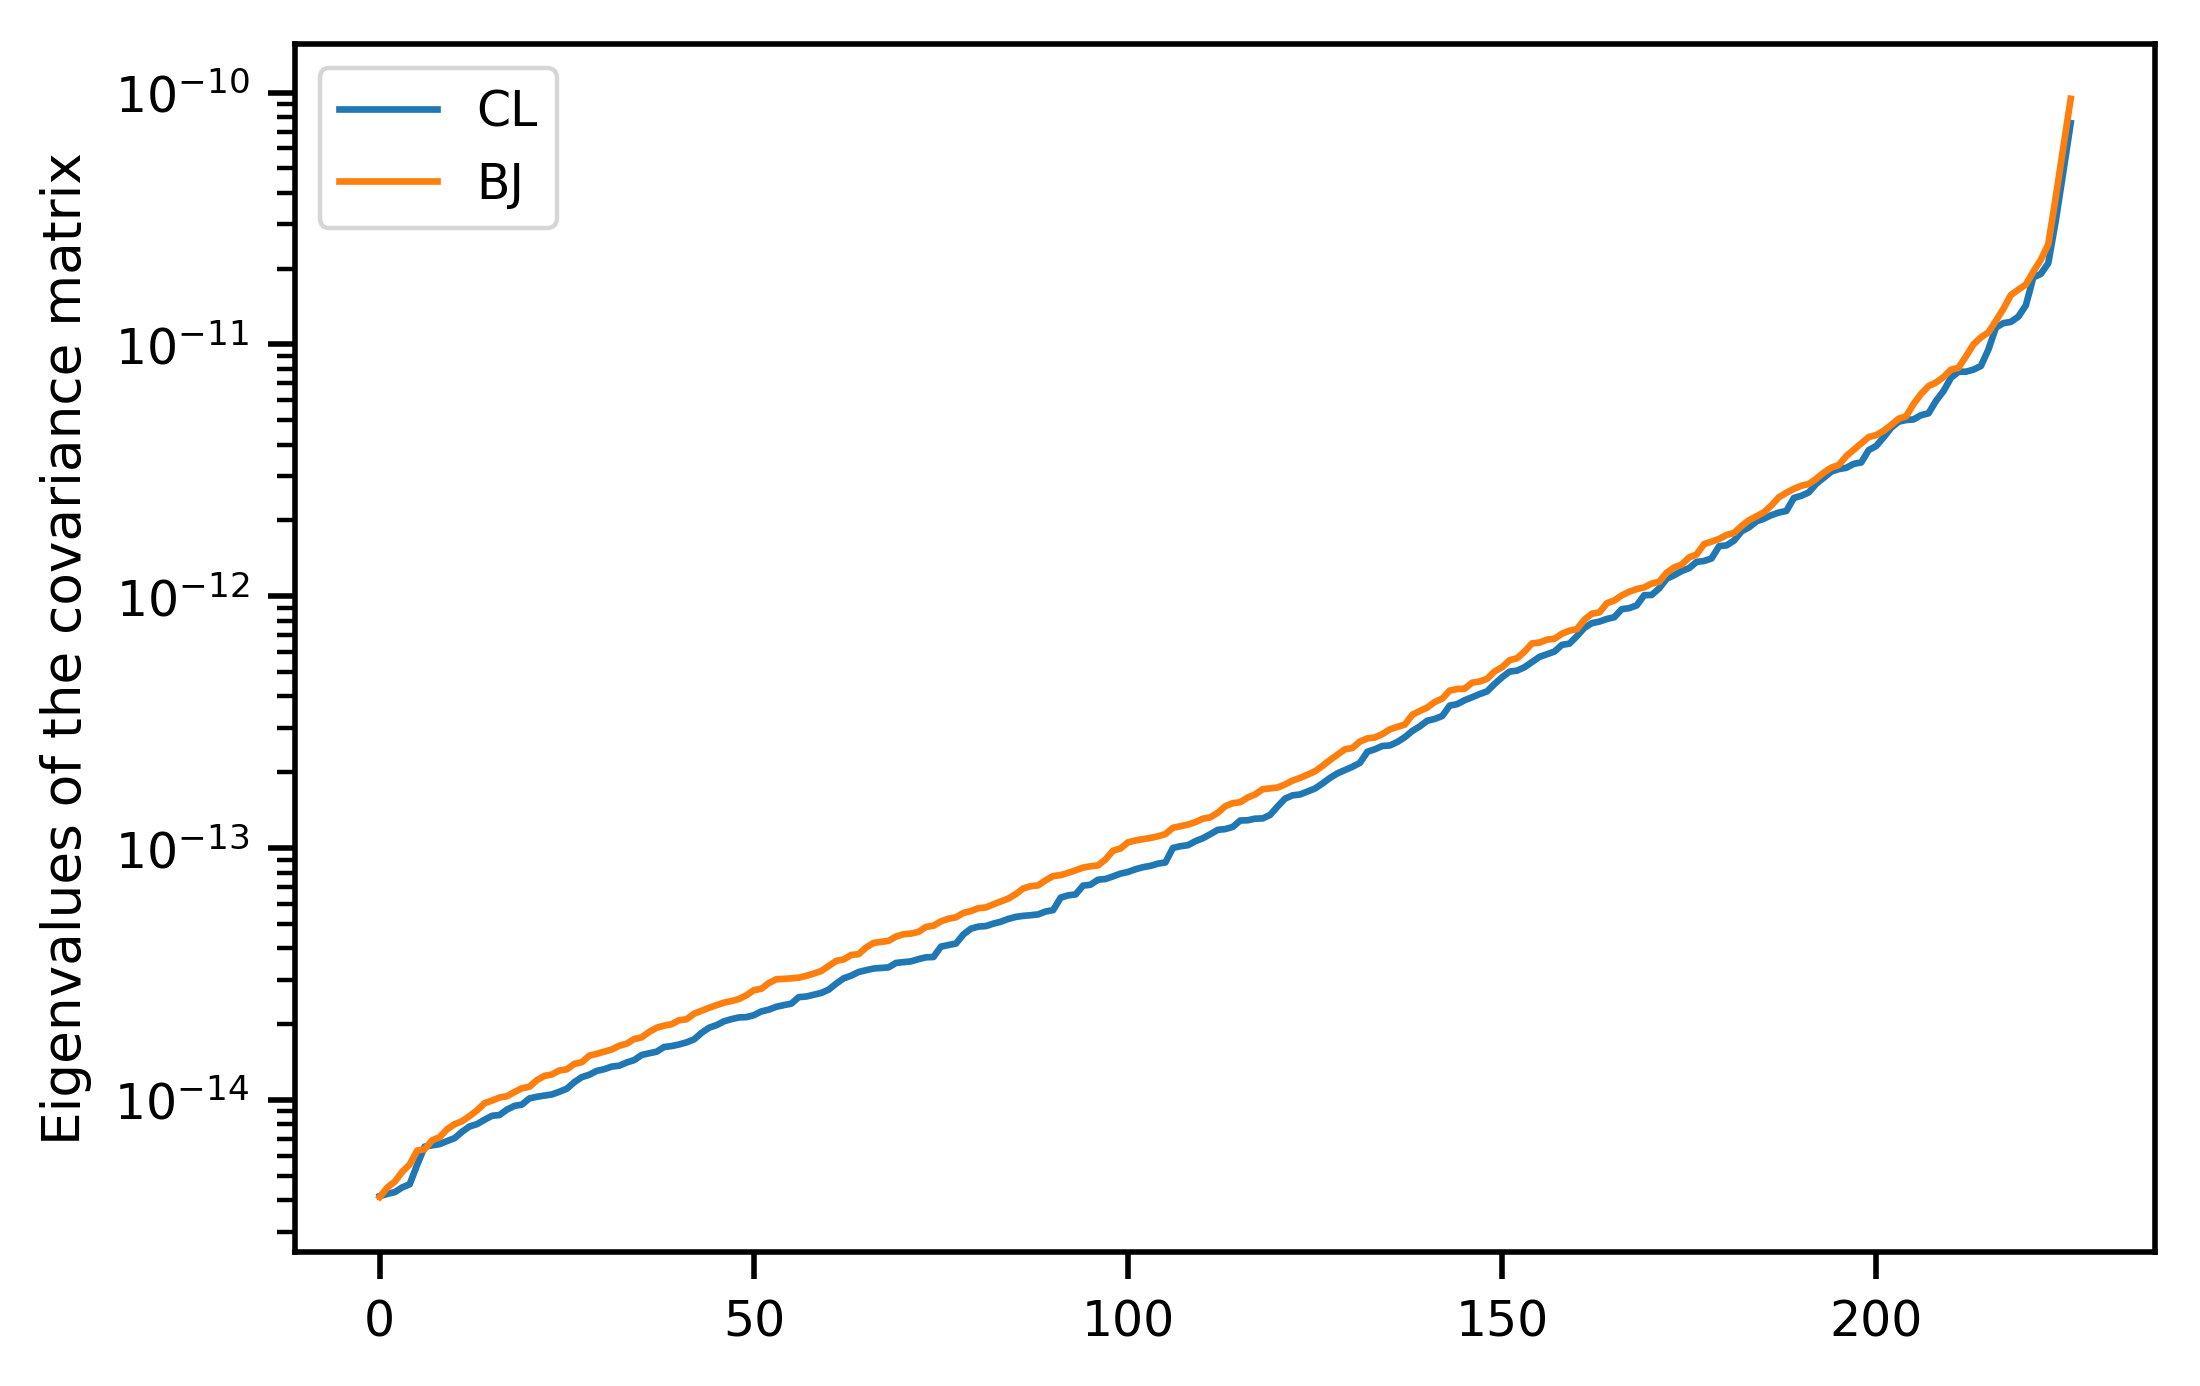
\includegraphics[width=0.9\columnwidth]{coveigen_BJ-CL.png}
\caption{A log plot showing the $227$ eigenvalues of two covariance matrices produced for cosmic shear for the Year 3 projection of the Dark Energy Survey. The blue curve is for CL and the orange one is for BJ. \label{fig:coveigen}}
\end{figure}

\figref{evector} shows an example of one of the eigenvectors, the one associated with the smallest eigenvalue. This low-eigenvalue mode picks up the differences between the correlation function at different angular scales (each vertical line delineates between two-point functions of shears in different tomographic bin pairs).

\begin{figure}
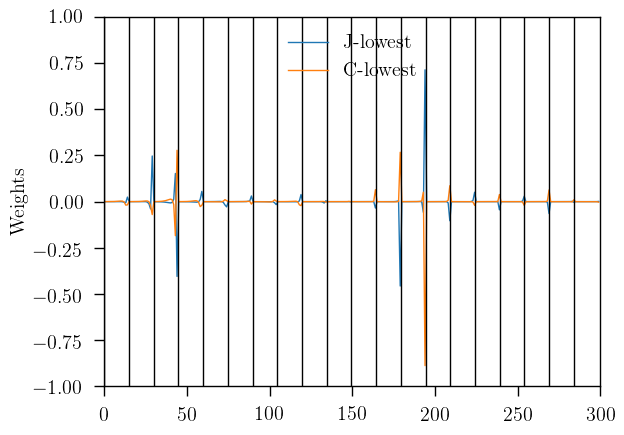
\includegraphics[width=0.9\columnwidth]{evector.png}
\caption{A simple scatter plot of elements of covariance matrices produced by two separate halo model codes. \label{fig:evector}}
\end{figure}

\subsection{Signal to noise}

Another way of analysing covariance matrices is by obtaining the signal-to-noise ratio (SNR). A simple way of achieving this is to note that the total SNR squared is

%Since the values of the data points vary by many orders of magnitude, the range of eigenvalues in Figure~\rf{evector} is a bit misleading. In addition, it is not clear which eigenvectors should be dropped: should it be chose with large eigenvalues (noise) or small ones (the noise is noisy)? Ideally, what we would like is to create a list of eigenvectors ordered in some way and drop the least important. This ties into the section below on Shrinkage. A very simple way to do this is to note that the total signal to noise squared is
\be
\left(\frac{S}{N}\right)^2 = \sum_{ij} D_i C^{-1}_{ij} D_j\
,\ee
where $D_i$ and $D_j$ are the data points and $C$ the covariance matrix. If $C$ were diagonal, then the eigenvectors would simply be the data points themselves, and we could estimate the SNR squared expected in each mode by simply computing $T_i^2/C_{ii}$ where $T_i$ is the theoretical prediction. Then we could throw out the modes with the lowest SNR. Since $C$ is not diagonal, we have to first diagonalise it and then order the values. So, we write the expected SNR squared as
%to do things a bit differently. Let's first define re-scaled data points
\bea
\left(\frac{S}{N}\right)^2 &=& \sum_{ij} T_i  C^{-1}_{ij} T_j\nonumber\\
&=& \sum_{i} \frac{v_i^2}{\lambda_i}
,\eea
where $\lambda_i$ are the eigenvalues of the covariance matrix, which is diagonalised with the unitary matrix $U$, and the eigenvectors are 
\be
v_i\equiv U_{ij}^t T_j
\ee
This makes it very clear which modes should be kept and which should be dropped. Modes $v_i$ for which $v_i^2/\lambda_i$ is very small can be discarded. 

After obtaining the SNR for our covariance matrix, we proceed to set the 50 lowest values to seven orders of magnitude lower, which is equivalent to increasing the noise (or decreasing the signal) of these modes. We then obtain a new covariance matrix with the corresponding modified SNR values. 


The parameter constraints for this method are shown in Figure~\rf{signalnoise}, where we note that the mean values are shifted about 12\% and 5\% for $\Omega_m$ and $\sigma_8$, respectively, with 17\% broader constraints for the former, when compared to the results with the original covariance, which tells us that the modes removed were essential for obtaining better constraints on these parameters. 

Another aspect that we must consider when applying this procedure is that the highest modes do not necessarily hold the most information for all of the parameters; this is evident when we analyse the SNR for each parameter individually. To illustrate this we take
\bea
\left(\frac{\partial S/\partial p_\alpha}{N}\right)^2 = \sum_{i} \frac{(\partial v_i / \partial p_\alpha)^2}{\lambda_i}
,\eea
with
\be
v_i^\alpha \equiv U_{ij}^t \frac{\partial T_j}{\partial p_\alpha}
,\ee
where $\partial /\partial p_\alpha$ is the derivative with respect to each parameter $\theta$. This produces the SNR for each parameter of interest. The importance of this procedure is illustrated in Figure~\rf{signalnoise_cuts}, where we can see that while the highest SNR for all the parameters does indeed correspond to those that hold most information for parameters $\Omega_m$ and $A_s$, this is not the case, however, for the intrinsic alignment parameters $A$ and $\eta$. As a result, we may end up losing constraining power over these parameters when we modify the lowest values of SNR. While this is apparent in the aforementioned figure, it is not very clear when looking at the resulting constraints on these parameters because the constraining power of the data over these parameters is not very strong (errors of about $100 \%$). As such, these results do not encourage us to use this method for identifying the most important elements of the covariance matrix.

\begin{figure}
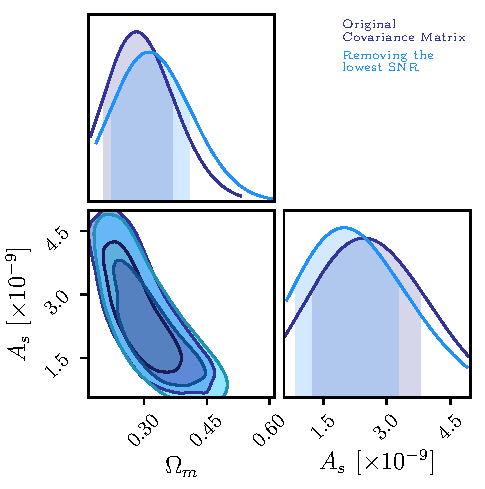
\includegraphics[width=0.9\columnwidth]{SN.pdf}
\caption{Constraints on cosmological parameters $\Omega_m$ and $A_s$ for the original DESY1 covariance matrix (in purple) and for a covariance matrix (in blue) obtained by setting fifty elements corresponding to the lowest SNR to a value nine orders of magnitude lower, in order to evaluate their contribution to parameter constraints. \label{fig:signalnoise}}
\end{figure}

\begin{figure}
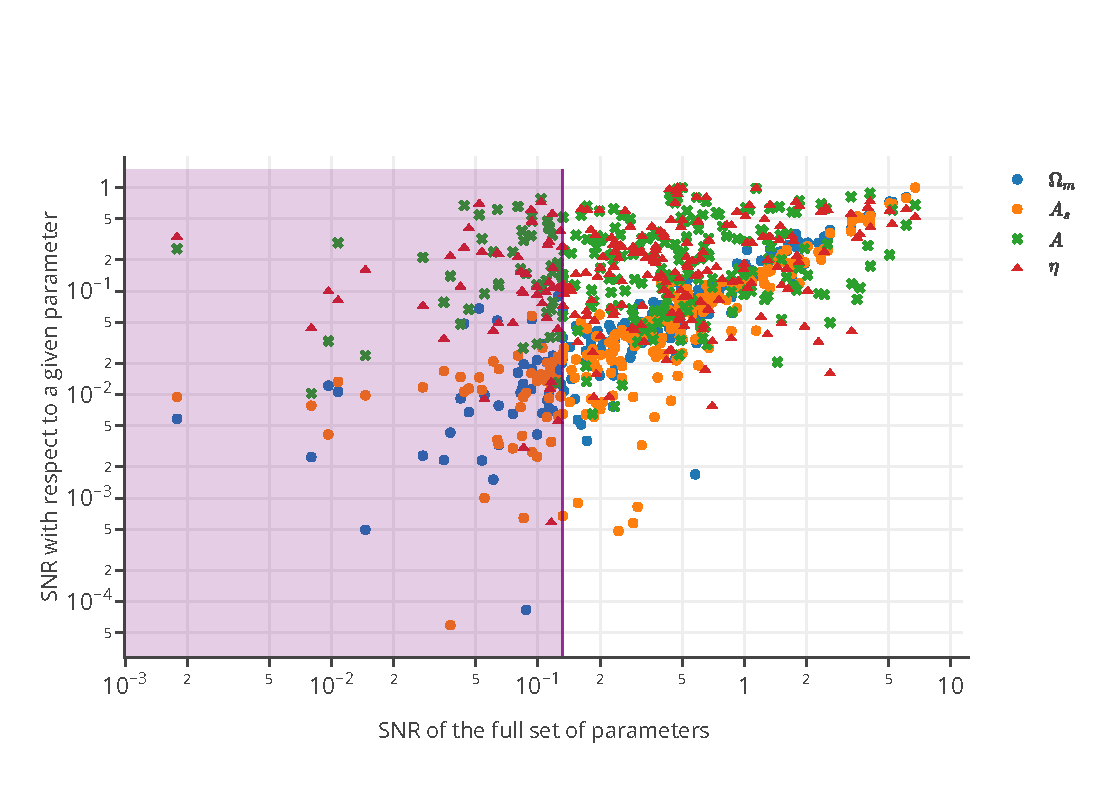
\includegraphics[width=1\columnwidth]{SNR_cuts.pdf}
\caption{Scatter plot for the relation between the signal to noise obtained with the covariance matrix for DESY1 for each parameter (x-axis) against that for the full set of parameters (y-axis). The derivatives are shown with respect to cosmological parameters $\Omega_m$ (blue) and $A_s$ (orange), and for the intrinsic alignment parameters $A$ (green) and $\eta$ (red). The purple rectangle spreads until the fiftieth lowest value of SNR, which corresponds to the values that were modified for parameter constraints. \label{fig:signalnoise_cuts}}
\end{figure}


\subsection{Parameter Estimation}

Ultimately, what matters is how well the likelihood does at extracting parameter constraints. Since most analyses assume a Gaussian likelihood, this boils down to how well the contours in parameter space agree when computing the $\chi^2$ using two different covariance matrices.

\subsection{Shrinkage}

There have been several methods proposed in the literature to compress the data vectors, extracting as much information as possible. Here we consider two: first compression at the map level~\citep{Alonso:2017hhj}, where linear combination of the tomographic maps are used. If there are 4 tomographic bins, an uncompressed analysis would require ten separate 2-point functions (or 20 for cosmic shear), whereas a compression scheme leads to just a few uncorrelated maps. If there were 3 such maps, then only three 2-point functions would need to be used for the likelihood analysis.

We characterize a given element in the data vector by its angular and tomographic indices: $a_i = a_{lm,\alpha}$ where $l,m$ denote the indices corresponding to given spherical harmonics and $\alpha$ is a given tomographic bin, or equivalently $a_i = a_\alpha(\vec\theta)$ in real space. The compression occurs in terms of tomographic bins, so that 
\be
b_\mu(\vec\theta) = \sum_{\alpha} F_{\mu\alpha} a_\alpha(\theta)
\ee
where the $F$'s are chosen \footnote{Note that this definition of $F$ differs from that in \citep{Alonso:2017hhj} in that it includes the inverse of the noise matrix.} so that the correlation functions of the $b$'s are diagonal in tomographic space:
\bea
w_{\mu\nu}(\theta) &=& \langle b_\mu(\vec\theta_1) b_\nu(\vec\theta_2)\rangle\vert_{\vert\vec\theta_1-\vec\theta_2\vert\in\theta}
\svs
&=& \delta_{\mu,\nu} w_{\mu}(\theta).
\eea
Usually with $N_t$ tomographic bins, one must consider $N_t(N_t+1)/2$ correlation functions, but -- due to the transformation that diagonalizes the elements -- there are only $N_t$ correlation functions to consider (for a given $\theta$). Even better, these can be ordered by the information they contain, so fewer than $N_t$can be used. In the example used in ~\citep{Alonso:2017hhj}, 16 tomographic bins were assumed, so that the standard treatment would require 136 correlation functions, but only 3 were needed in order to extract accurate constraints. 

This method suggests a way of extracting the most important pieces of the full covariance matrix $C$. We simply compute the covariance matrix of the $w_{\mu}$ in terms of $C$ and keep only the most important terms. That is,
\bea
C^b_{\mu\nu} &\equiv& \langle (w_{\mu} -\bar w_\mu)\,(w_{\nu} -\bar w_\nu)\rangle
\svs
&=& \sum_{\alpha\alpha'\beta\beta'} F_{\mu\alpha}F_{\mu\alpha'}\, F_{\nu\beta}F_{\nu\beta'}\, C_{\alpha\alpha'\beta\beta'} .
\eea
Here the angular indices have been suppressed (there are two of them, one for each $w_\mu$), but the full tomographic complexity has been retained. The covariance matrix on the right includes a total of $N_t^2 \times N_t^2$ terms (some of which are equal because of symmetry) corresponding to all possible pairs of two-point functions. But $C^b$ on the right contains only $N_t^2$ elements, and again these are ordered, so we can use only a subset of them. In the simplest case, where only one linear combination is needed so $\mu=\nu=1$, a single number (for each pair of angular bins) captures all the relevant information from the full covariance matrix.

\subsubsection{2-Point Correlation Function}

The second compression takes place at the 2-point level~\citep{Zablocki:2015zcm}, with the compressed data vector containing linear combinations of the many 2-point functions. In principle, this might work with only $N_p$ 2-point functions where $N_p$ is the number of parameters varied, and each mode, or linear combination, contains all the information necessary about the parameter of interest. 

For each parameter $p_\alpha$ that is varied, one captures a single linear mode
\be
y_\alpha = U_{\alpha i} D_i
\ee
where $D_i$ are the data points and the coefficients are defined as
\be \label{eq:compression_scheme}
U_{\alpha i} \equiv \frac{\partial T_j}{\partial p_\alpha} \, C^{-1}{}_{ji}
\ee
where $T_j$ is the theoretical prediction for the data point $D_j$.
The now much smaller data set $\{y_\alpha\}$, which contains as few as $N_p$ data points, carries with it its own covariance matrix, with which the $\chi^2$ can be computed for each point in parameter space. Propagating through shows that this covariance matrix is related to the original $C_{ij}$ via
\be
C_{\alpha\beta} = U_{\alpha i} C_{ij} U^t_{j\beta}.
\ee
To take an example from the full DESY1 for cosmic shear, $C_{ij}$ is a $400 \times 400$ matrix, while the number of parameters needed to specify the model is only 16, so $C_{\alpha\beta}$ is a $16\times 16$ matrix. We have apparently captured from the initial set of $(400 \times 401)/2 = 80,200$ independent elements of the covariance matrix a small subset (only 136 in this case) of linear combinations of these 80k elements that really matter. If two covariance matrices give the same set of $C_{\alpha\beta}$, we do not care whether any of the other eighty thousand elements differ from one another.

In our case, our covariance matrix is  $227 \times 227$, which we then reduce to $16 \times 16$ elements. Figure \textcolor{red}{include figure} compares the constraints obtained for the compressed covariance and data with the full one, for $\Omega_m$ and $\sigma_8$.  \textcolor{red}{Include plots and talk about constraints.} While this compression does not speed up calculations, it is encouraging to see that we can compress matrices of any size without losing a significant amount of information on the parameters of our models. 

One relevant point in this analysis is at which point to take the derivative of each parameter. When we wish to compare the results of our compression scheme with those obtained with the full covariance matrix and data set, it is important to derivate each parameter at their respective mean value (obtained by performing the analysis with the full covariance matrix). The shape and variance of the posterior is not dependent on the derivative, but the best fit value shifts according to the point where the derivative was taken.

We also apply this methodology to comparing the covariance matrices of interest, i. e. CL and BJ. In order to do this, we take two different approaches: first, we assume that $U_{\alpha, i}$ is the same for both covariance matrices and we calculate it with BJ. The second approach is that each compression scheme must use the original covariance matrix that will be compressed, so that $U_{\alpha, i}$ will be different for each covariance matrix. Figure~\rf{correlation} was obtained for the first method, it shows the correlation matrix for BJ and CL, and that of the difference between them; we find this figure important because we can clearly see the difference between the two matrices by simply looking at only $(16 \times 17)/2$ elements, as opposed to having to analyse the larger correlation matrix for the full covariance matrices. It is also crucial that the matrices used for comparison here are those obtained via the same compression scheme, so that we can be sure that their differences are indeed only related to the differences in the original matrices.

\subsubsection{Cool section name here}

While the compression scheme is \textcolor{red}{good?}, it is not devoid of problems, the most concerning one being that we cannot recover the original covariance matrix the compressed one. Our motivation is to have an invertible transformation so that we are able to switch between a compressed and the full covariance. In order to do this, we start off with the compression scheme presented in Eq. \ref{eq:compression_scheme}, which will serve as the basis for a rotation matrix $W_\alpha$. We then use the Gram-Schmidt decomposition to create $227 - N_p$ vectors orthonormal to $U_{\alpha}$, thus obtaining a unitary $227 \times 227$ matrix. We then have,
\be
C'_{\alpha\beta} = W_{\alpha i} C_{ij} W^t_{j\beta}.
\ee
 When this transformation is applied to the original matrix, $C_{ij}$, the first $N_p \times N_p$ elements of the new matrix will be the same as we had in $C_{\alpha\beta}$. Since our transformation spreads out the information contained in the compressed matrix, the relevant values for parameter estimation will be contained in the first $N_p$ rows and columns of the new covariance matrix. This means that we will have $N_p \left( 2 \times 227 - N_p \right)$ important elements, which is about an order of magnitude less than in the case of the full covariance matrix.
 
 
 
 \begin{table}
\centering
\begin{tabular} { l c} 
\hline
\hline
Added error	& Standard deviation 	\\ \hline \\
$0 - 20 \% $		& 	$< 5$	\\
$20 - 40 \% $		& 	$< 20$	\\
$> 50 \% $		& 	$> 20$	\\ [1ex]
\hline
\hline
\end{tabular}
\caption{The first column is the introduced error to the relevant elements of the rotated covariance matrix for $\Omega_m$. The introduced error corresponds to the an arbitrary increase in each element in the first row and first column of the rotated covariance matrix }
\label{tab:error_budget}
\end{table}





\begin{figure}
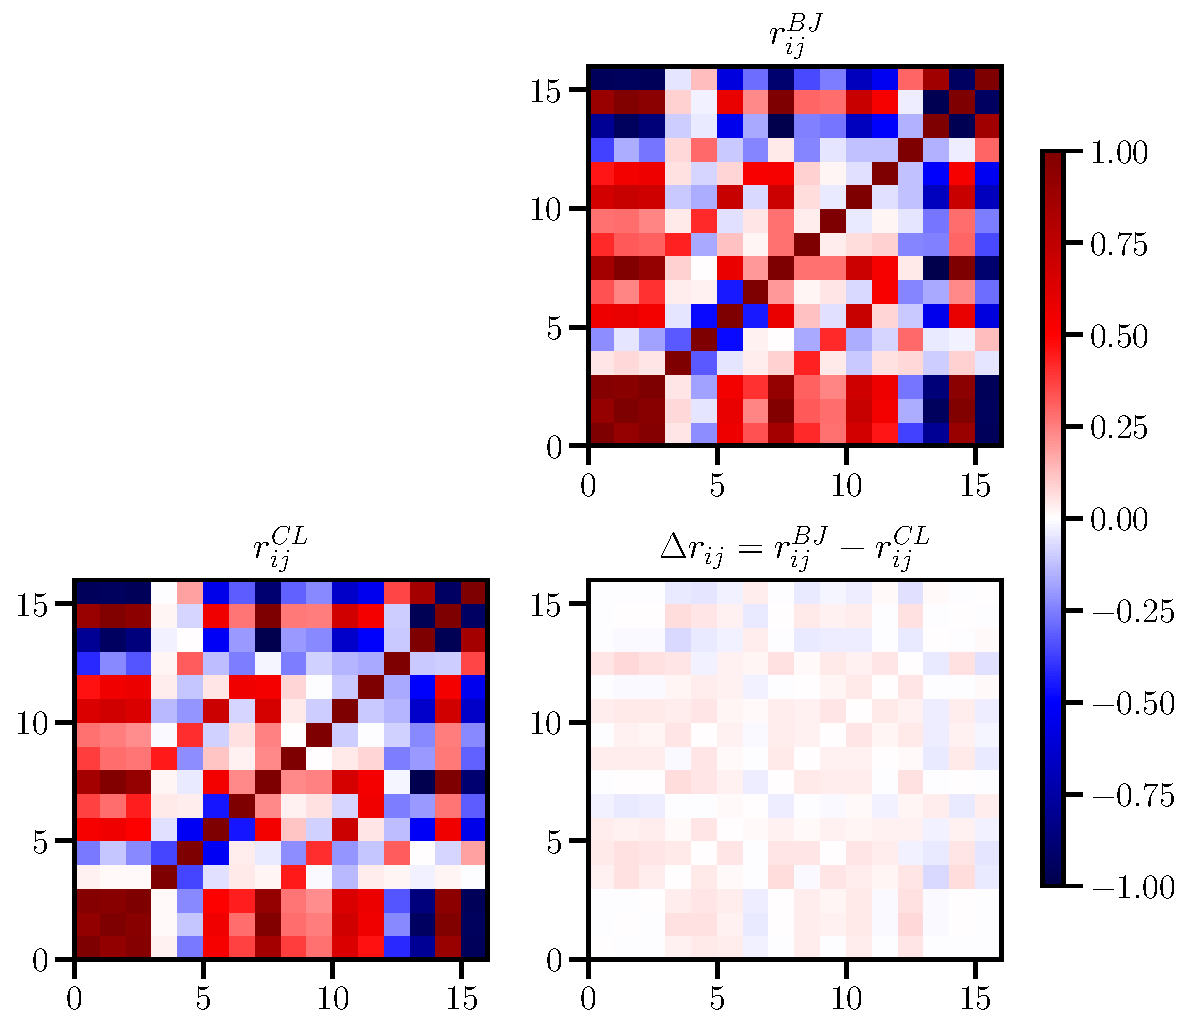
\includegraphics[width=0.9\columnwidth]{Correlation_compression.pdf}
\caption{The upper right and lower left plots display the correlation matrix for BJ and CL respectively, while the lower right is the difference between the two. \label{fig:correlation}}
\end{figure}


% ----------------------------------------------------------------------

\section{Results}
\label{sec:results}



% ----------------------------------------------------------------------

\section{Discussion}
\label{sec:discussion}



% ----------------------------------------------------------------------

\section{Conclusion}
\label{sec:conclusion}



% ----------------------------------------------------------------------

\subsection*{Acknowledgments}

%%% Here is where you should add your specific acknowledgments, remembering that some standard thanks will be added via the \code{desc-tex/ack/*.tex} and \code{contributions.tex} files.

%This paper has undergone internal review in the LSST Dark Energy Science Collaboration. % REQUIRED if true


 % Standard papers only: author contribution statements. For examples, see http://blogs.nature.com/nautilus/2007/11/post_12.html

% This work used TBD kindly provided by Not-A-DESC Member and benefitted from comments by Another Non-DESC person.

% Standard papers only: A.B.C. acknowledges support from grant 1234 from ...

The DESC acknowledges ongoing support from the Institut National de Physique Nucl\'eaire et de Physique des Particules in France; the Science \& Technology Facilities Council in the United Kingdom; and the Department of Energy, the National Science Foundation, and the LSST Corporation in the United States.  DESC uses resources of the IN2P3 Computing Center (CC-IN2P3--Lyon/Villeurbanne - France) funded by the Centre National de la Recherche Scientifique; the National Energy Research Scientific Computing Center, a DOE Office of Science User Facility supported by the Office of Science of the U.S.\ Department of Energy under Contract No.\ DE-AC02-05CH11231; STFC DiRAC HPC Facilities, funded by UK BIS National E-infrastructure capital grants; and the UK particle physics grid, supported by the GridPP Collaboration.  This work was performed in part under DOE Contract DE-AC02-76SF00515.
 % also available: key standard_short

% This work used some telescope which is operated/funded by some agency or consortium or foundation ...

% We acknowledge the use of An-External-Tool-like-NED-or-ADS.

%{\it Facilities:} \facility{LSST}

% Include both collaboration papers and external citations:
\bibliography{main,lsstdesc}

\end{document}

% ======================================================================
